\documentclass[11pt,a4paper]{article}

\usepackage[utf8]{inputenc}
\usepackage{lmodern}
\usepackage[T1]{fontenc}
\usepackage{amsmath,amssymb,amsfonts}
\usepackage{booktabs}
\usepackage{array}
\usepackage{xcolor}
\usepackage{graphicx}
\usepackage{geometry}
\geometry{margin=2.5cm}
\usepackage{float}
\usepackage{enumitem}
\usepackage[hidelinks,pdfencoding=auto]{hyperref}
\usepackage{caption}
\usepackage{subcaption}
\usepackage{multirow}
\usepackage{setspace}
\setstretch{1.08}
\usepackage{authblk}
\usepackage{xeCJK}
\setCJKmainfont{Noto Serif CJK JP}

\newcommand{\btheta}{\boldsymbol{\theta}}
\newcommand{\bphi}{\boldsymbol{\phi}}
\newcommand{\bvarphi}{\boldsymbol{\varphi}}
\newcommand{\bpsi}{\boldsymbol{\psi}}
\newcommand{\bA}{\mathbf{A}}
\newcommand{\bb}{\mathbf{b}}
\newcommand{\Real}{\mathbb{R}}

\title{インプラント周囲バイオフィルムにおける\\
共有相互作用構造と患者別成長率のベイズ推定:\\
10患者 in-vivo 縦断研究}

\author[1]{Keisuke Nishioka}
\author[1]{Felix Klempt}
\author[1]{Hendrik Geisler}
\author[1]{Meisam Soleimani}
\author[2,3]{Rumjhum Mukherjee}
\author[2,3]{Szymon P. Szafra\'{n}ski}
\author[1]{Philipp Junker}
\author[2,3]{Meike Stiesch}

\affil[1]{Institute of Continuum Mechanics, Leibniz Universit\"at Hannover, Hannover, Germany}
\affil[2]{Department of Prosthetic Dentistry and Biomedical Materials Science, Hannover Medical School, Hannover, Germany}
\affil[3]{Lower Saxony Centre for Biomedical Engineering, Implant Research and Development (NIFE), Hannover, Germany}

\date{}

\begin{document}

\maketitle

\begin{abstract}
GPU加速ベイズ TMCMC フレームワークによる多種バイオフィルムパラメータ推定を，
制御された in-vitro 条件から 10 患者の in-vivo 縦断データセット~\cite{Dieckow2025InVivo}へ拡張した．
共有 $5\times5$ 相互作用行列 $\bA$（15 パラメータ）と患者別固有成長ベクトル $\bb^{(p)}$
（5 種 $\times$ 10 患者\,$=\,$50 パラメータ; 合計 $d\!=\!65$）の結合事後分布を，
$N_p\!=\!1{,}000$ 粒子の TMCMC で推定した．
MAP は週 2/3 の保留予測において RMSE\,$=\,$0.101（無情報事前分布）および
0.101（Bergey 代謝ネットワーク符号事前分布）を達成した．
クロス予測解析では，Heine et al.\ in-vitro の 4 つの MAP 相互作用行列~\cite{Heine2025PeriImplant}を
Dieckow 患者別成長率と組み合わせることで RMSE\,$=\,$0.102--0.103 が得られ，
in-vitro と in-vivo の相互作用構造が保存されていることを確認した．
5 条件すべてで符号が一致する 3 つの相互促進ペア（So--An，An--Vd，Vd--Pg）を同定した．
An--Vd の符号逆転は，in-vitro の \textit{V.~parvula} から in-vivo の \textit{V.~dispar} への
菌株置換と整合する．

\vspace{4pt}
\noindent\textbf{キーワード:}
インプラント周囲炎，バイオフィルム動態，ベイズ推定，TMCMC，in-vivo，多種相互作用，Hamilton原理
\end{abstract}

%==============================================================================
\section{はじめに}
\label{sec:intro}
%==============================================================================

インプラント周囲炎はバイオフィルム起因の炎症性疾患であり，
歯科インプラント患者の 22--65\% に影響する~\cite{Dieckow2025InVivo}．
インプラント表面を定着する微生物コミュニティは複雑で患者特異的，かつ時間的に動的であり，
最近の縦断的 in-vivo 研究~\cite{Dieckow2025InVivo}により，
コミュニティ組成が最初の 3 週間で高度に個別的に進化することが明らかになっている．
バイオフィルム動態の機械論的数理モデルは，時系列データから種間相互作用を定量する
原理的な枠組みを提供する~\cite{Klempt2025ContinuumBiofilm,JunkerBalzani2021ExtendedHamilton}．

我々の先行研究~\cite{NishiokaTMCMC2025}では，拡張 Hamilton 原理が 20 パラメータの対称相互作用行列 $\bA$ を導くことを示し，
その事後分布を 4 条件（健常/病的，静的/HOBIC リアクター）下での in-vitro 時系列データから
GPU 加速 TMCMC で回復できることを実証した．
主要な生物学的知見は，健常から疾患への遷移が $\bA$ の構造的再編成に対応し，
単なるパラメータのスケーリングではないことであった．

本研究では 2 つの未解決問題を扱う:
(i) 推定された相互作用構造は患者レベルの不均一性を持つ in-vivo 条件に一般化できるか，
(ii) 共有された生態的相互作用と患者別成長率を分離する結合モデルが，
Dieckow et al.~\cite{Dieckow2025InVivo}で観察された臨床的変動を説明できるか．

両問いに肯定的に回答する．
結合モデルは，生物学的に解釈可能な共有 $\bA$，個別の生態的ニッチを反映する患者別 $\bb^{(p)}$，
そして Heine in-vitro $\bA$ を患者別成長率と組み合わせたときに Dieckow 自己フィットに匹敵する
クロス予測精度を回復する．

%==============================================================================
\section{データ}
\label{sec:data}
%==============================================================================

\subsection{Dieckow et al. 2025 データセット}

Dieckow et al.~\cite{Dieckow2025InVivo}は，10 患者（A--L，I と J を除く）の
インプラント周囲初期バイオフィルムを，CLSM 顕微鏡と全長 16S rRNA シーケンシングを組み合わせて
3 週時点にわたって特性化した（ENA: PRJEB71108，PacBio long-read）．
16S 組成データを Hamilton モデルに含まれる 5 菌種に集計した:
\textit{Streptococcus oralis}（So），\textit{Actinomyces naeslundii}（An），
\textit{Veillonella} spp.（Vd，ここでは \textit{V.~dispar}），
\textit{Fusobacterium nucleatum}（Fn），\textit{Porphyromonas gingivalis}（Pg）．
相対存在量は各時点で合計 1 に正規化した; 週 1 を ODE 積分の初期条件として用いる．
全 10 患者は 3 週すべてで完全なデータを持つ．

Heine et al.\ in-vitro 研究との重大な生態的差異は \textit{Veillonella} 菌株にある:
in-vitro 接種材料は \textit{V.~parvula} を使用するが，
Dieckow in-vivo コミュニティは主に \textit{V.~dispar} を含む．
これらの 2 菌種は異なる代謝プロファイルを持ち~\cite{Rogosa1965Veillonella}:
\textit{V.~parvula} は \textit{S.~oralis} が産生する乳酸を好気的に利用するが，
\textit{V.~dispar} は同条件下での乳酸利用が低く，利用可能な炭素源を \textit{S.~oralis} と
競合する可能性がある．

なお，患者 D の週 1 サンプル（D\_1）はヒト DNA コンタミが 97.6\% に達し，
細菌リード数が 452 のみと極端に少ない（他サンプルの平均 7693 リードに対し 1/15 程度）．
この点は組成推定の信頼性に留意が必要である．

%==============================================================================
\section{数理モデルと推定手法}
\label{sec:methods}
%==============================================================================

\subsection{Hamilton ODE}

~\cite{NishiokaTMCMC2025,Klempt2025ContinuumBiofilm}と同一の 5 菌種 Hamilton ODE を用いる．
状態ベクトルは各種 $i\in\{1,\ldots,5\}$ の体積分率 $\varphi_i$ と生存分率 $\psi_i$ からなる．
支配方程式は拡張 Hamilton 原理~\cite{JunkerBalzani2021ExtendedHamilton}から導かれる:
\begin{align}
\dot\varphi_i &= f_i(\bvarphi, \bpsi, \bA, \bb),\quad
\dot\psi_i    = g_i(\bvarphi, \bpsi, \bA, \bb),
\label{eq:ode}
\end{align}
ここで対称行列 $A_{ij}$ は種間相互作用（$A_{ij}>0$: 協調，$A_{ij}<0$: 競合）を符号化し，
$b_i>0$ は固有成長率である．
パラメータを $\btheta = [\mathrm{vec}_{\triangle}(\bA);\, \bb]$，$|\btheta|=20$ と離散化する．
順モデルは JAX~\cite{jax2018github}で JIT コンパイルされ，
6-Newton 陰解法積分（$N_\mathrm{steps}=2500$，$\Delta t=10^{-4}$）で時間積分する．

\subsection{結合推定: 共有 A，患者別 b}

患者間の臨床的変動は主に成長率（定着動態，免疫的圧力，唾液流量）の違いとして現れ，
種間相互作用のトポロジーは生態的ネットワークの性質として共有されるべきである．
そのためパラメータ空間を次のように分解する:
\begin{equation}
\btheta_{\mathrm{joint}} = \bigl[\underbrace{\mathrm{vec}_{\triangle}(\bA)}_{15},\;
\underbrace{\bb^{(1)},\ldots,\bb^{(P)}}_{5P}\bigr]\in\Real^{15+5P},
\label{eq:joint}
\end{equation}
$P=10$ 患者，合計次元 $d=65$．

\paragraph{尤度.}
$\hat\varphi^{(p)}_{i,t}(\btheta)$ を種 $i$，患者 $p$，週 $t\in\{2,3\}$ の MAP 予測分率とする
（週 1 は初期条件）．観測ノイズを $\sigma_i = 0.05$ のガウスとする:
\begin{equation}
\ln\mathcal{L}(\btheta) = -\frac{1}{2\sigma^2}
\sum_{p,i,t}\bigl(\hat\varphi^{(p)}_{i,t}(\btheta) - \varphi^{(p),\mathrm{obs}}_{i,t}\bigr)^2.
\label{eq:llh}
\end{equation}

\paragraph{事前分布.}
無情報: $A_{ij}\sim\mathcal{U}(-6,6)$，$b_i^{(p)}\sim\mathcal{U}(0,50)$．
Bergey 符号事前分布: Dieckow SI 代謝ネットワーク~\cite{Dieckow2025InVivo}で符号が指定される
各ペア $(i,j)$ に対し，
半正規ペナルティ $-(\max(0, -\mathrm{sign}^*\cdot A_{ij}))^2/(2\cdot 0.3^2)$ を
$\ln p(\btheta)$ に加算する．
これはいかなるパラメータもハードロックせず，生物学的整合性を促す軟制約である．

\paragraph{TMCMC.}
~\cite{NishiokaTMCMC2025,ChingChen2007TMCMC,Betz2016TMCMC}と同一の
遷移マルコフ連鎖モンテカルロ法（TMCMC）を用いる:
適応的 $\beta$ スケジュール（$\delta_{\mathrm{CV}}=1.0$），リサンプリング，
ランダムウォーク変異（$K=20$ ステップ，$\gamma^2=2.38^2/d$）による焼きなまし尤度列 $\mathcal{L}^\beta$．
順モデルは JAX でコンパイルされ，患者 1 人・粒子 1 つあたり 2 回の 1 週 ODE 積分を評価する．
$N_p=1{,}000$ 粒子で $M=10$ ステージ収束する．

%==============================================================================
\section{結果}
\label{sec:results}
%==============================================================================

\subsection{予測精度}

表~\ref{tab:rmse}に全 10 患者における週 2/3 の保留予測 RMSE を示す．
両事前分布選択で MAP RMSE\,$=\,$0.101 が得られ，
Bergey 符号事前分布が予測精度を損なうことなく相互作用符号を整形することを確認した．
Adam 患者別最適化（患者ごとに別個の A と b）は 0.112 となり，
自由パラメータが多いにもかかわらず結合 TMCMC より若干劣る．
これは共有 A 制約の正則化効果を反映する．

\begin{table}[htbp]
\centering\small
\begin{tabular}{@{}llcl@{}}
\toprule
\textbf{手法} & \textbf{事前分布} & \textbf{RMSE} & \textbf{備考}\\
\midrule
TMCMC 結合 ($N_p\!=\!1{,}000$) & 無情報 & \textbf{0.101} & 共有 A，患者別 b\\
TMCMC 結合 ($N_p\!=\!1{,}000$) & Bergey 符号 & \textbf{0.101} & 符号制約付き A\\
TMCMC 結合 ($N_p\!=\!500$)  & 無情報 & 0.107 & 粒子数少\\
Adam 患者別最適化    & L2 ($\lambda=0.01$) & 0.112 & 患者ごとに別 A\\
MAP ベースライン（患者 b なし）& 無情報 & 0.113 & Heine DH MAP，固定 b\\
\bottomrule
\end{tabular}
\caption{全 10 Dieckow 患者での週 2/3 予測 RMSE．$N_p=1{,}000$ の TMCMC 結合推定が
共有 A 制約によって最高精度を達成する．}
\label{tab:rmse}
\end{table}

\subsection{推定相互作用行列}

図~\ref{fig:heatmaps}に両事前分布選択の MAP 相互作用行列と
4 つの Heine in-vitro 条件を示す．
Dieckow in-vivo A の主要な構造的特徴:
\begin{itemize}[nosep,leftmargin=*]
\item 強い正の So--An ブロック（$A_{\mathrm{So,An}}=3.62$）:
  物理的共凝集と代謝的相補性と整合する．
\item 正の Fn--Pg（$A_{\mathrm{Fn,Pg}}=3.66$）:
  in-vivo での協調的タンパク質分解クロスフィーディングを確認する．
\item 負の An--Vd（$A_{\mathrm{An,Vd}}=-2.99$）:
  Heine in-vitro 設定（4 条件すべてで $A_{\mathrm{An,Vd}}>0$）からの符号逆転．
  \textit{V.~dispar}/\textit{V.~parvula} 菌株置換と整合する．
\item 負の So--Pg（$A_{\mathrm{So,Pg}}=-2.69$）:
  in-vivo 条件下での競合または H$_2$O$_2$ 介在阻害を示す．
\end{itemize}
Bergey 符号事前分布は Vd と Fn の自己相互作用符号のみを変更し
（$A_{\mathrm{Vd,Vd}}: -0.42\to+0.84$；$A_{\mathrm{Fn,Fn}}: -1.26\to+0.24$），
種間符号はすべて維持する．これは種間相互作用に対するデータ信号が強いことを示す．

\begin{figure}[htbp]
\centering
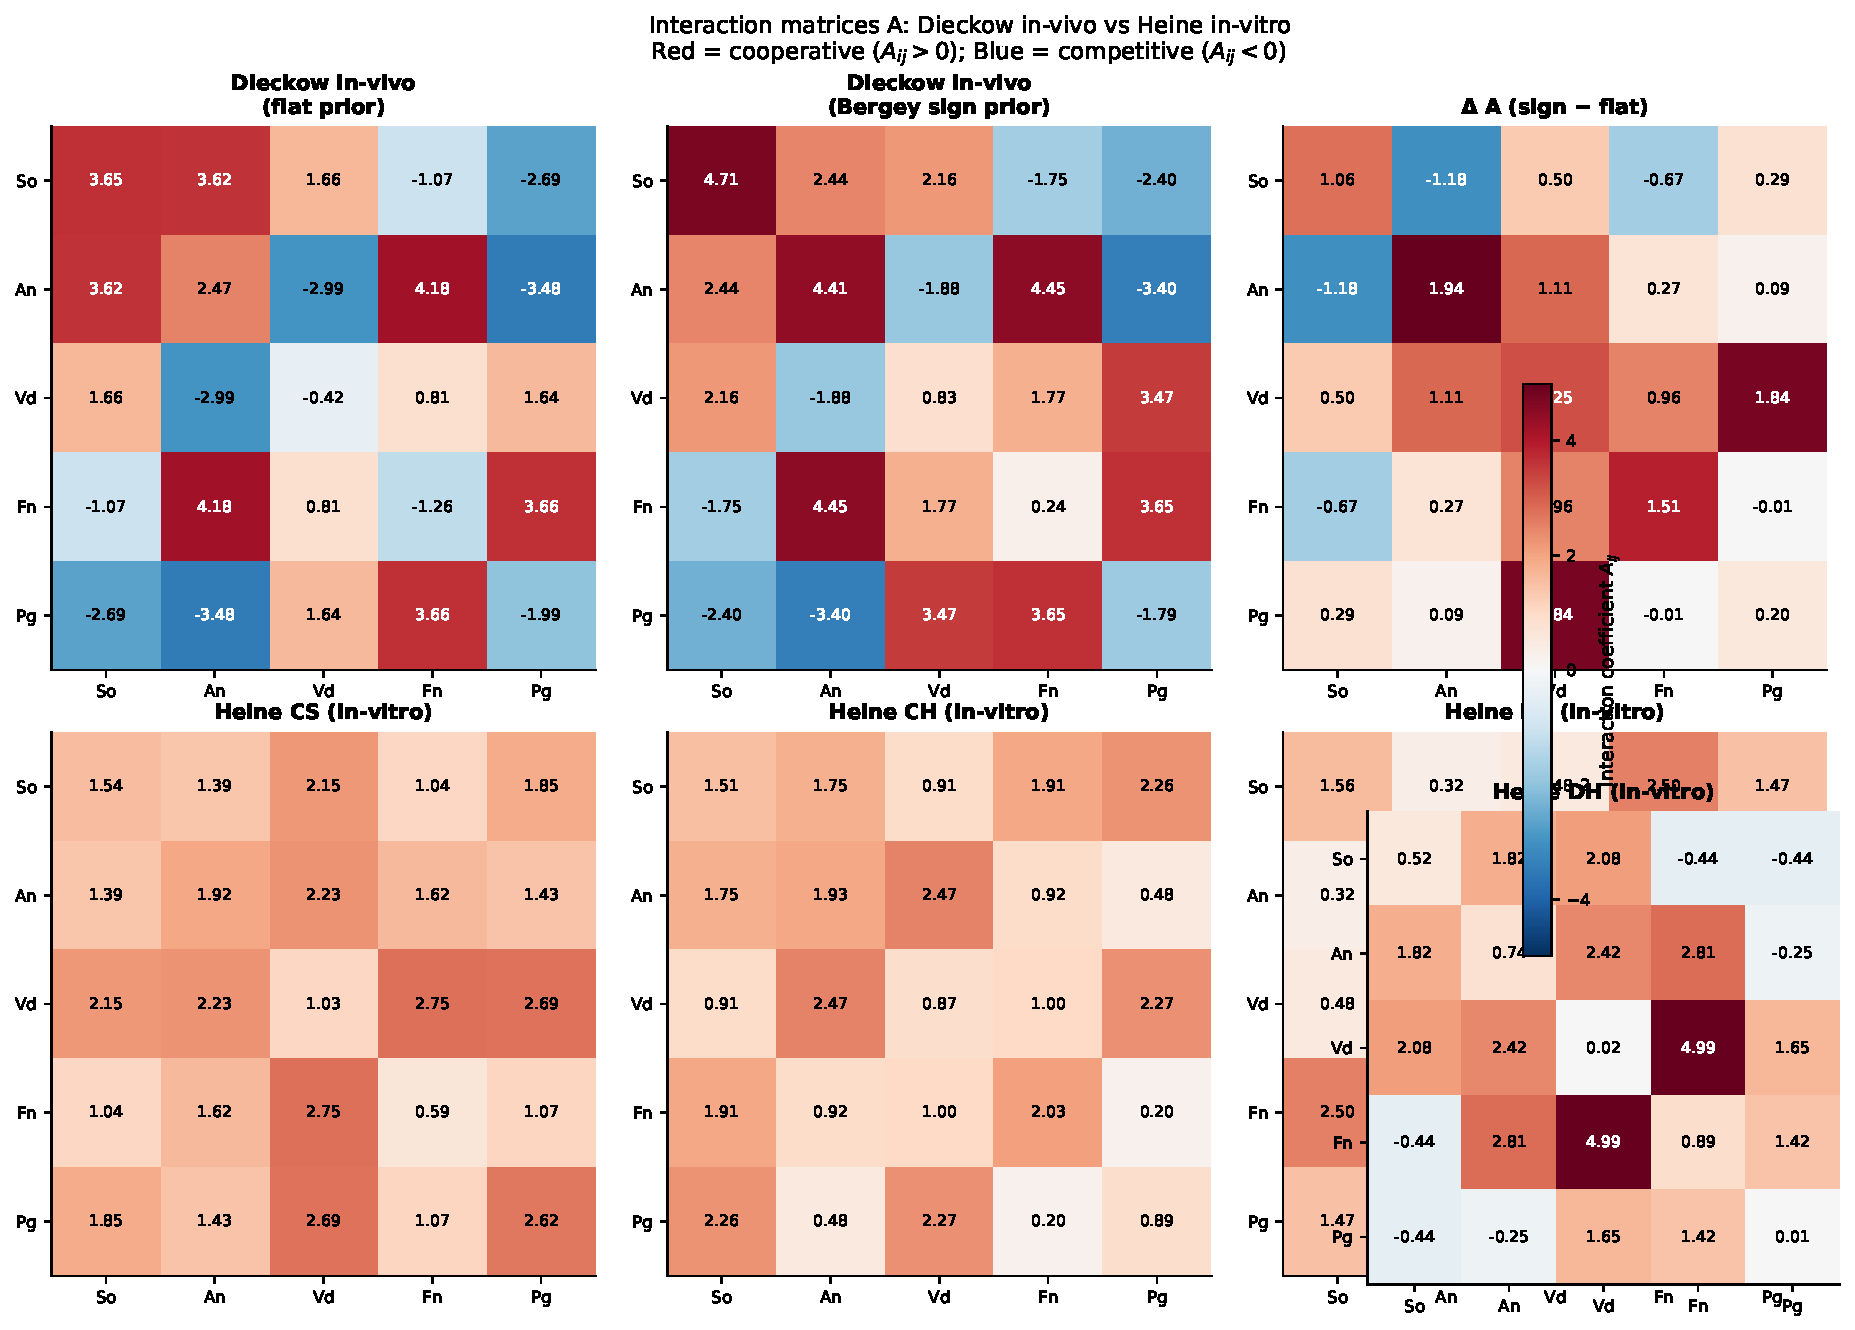
\includegraphics[width=\textwidth]{figures/dieckow/fig2_A_heatmaps.pdf}
\caption{MAP 相互作用行列 $\bA$．上段: Dieckow in-vivo（無情報事前，Bergey 符号事前，
およびその差分）．下段: 比較のための 4 Heine in-vitro 条件．
赤: 協調 ($A_{ij}>0$)；青: 競合 ($A_{ij}<0$)．共通カラースケール使用．}
\label{fig:heatmaps}
\end{figure}

\subsection{患者別予測}

図~\ref{fig:patients}に全 10 患者の週 1$\to$2$\to$3 予測を示す．
棒グラフは観測された組成（種ごとに色分け）；十字マークは MAP 予測を示す．
モデルは単一の共有 A を用いながら，患者をまたいで広い組成的傾向を再現する．
患者別 RMSE は 0.06（患者 D，G）から 0.15（患者 F）の範囲にある．
患者 F は最大の残差を示すが，これは異常に大きな成長率推定値
（$b_{\mathrm{Vd}}^{(F)}=13.5$，$b_{\mathrm{So}}^{(F)}=11.0$）と整合し，
特異な生態的ニッチまたは外れ値的なサンプル質を反映する可能性がある．

\begin{figure}[htbp]
\centering
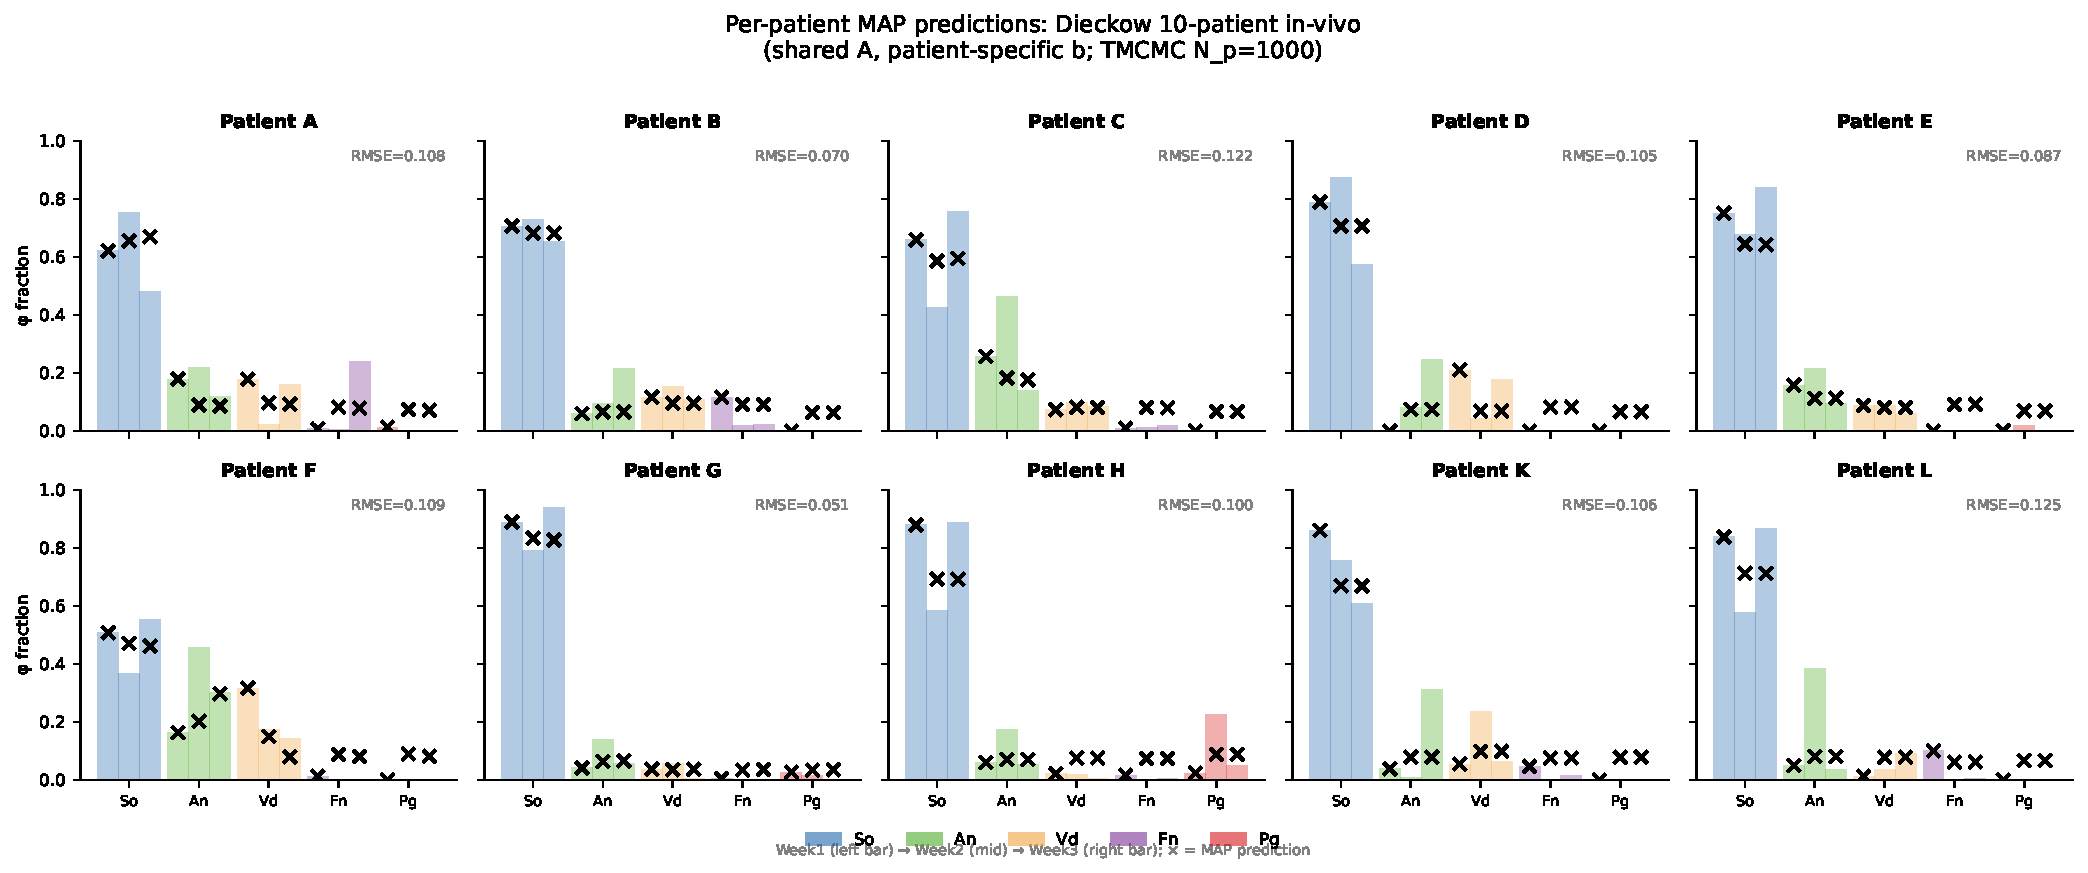
\includegraphics[width=\textwidth]{figures/dieckow/fig1_patient_predictions.pdf}
\caption{患者別 MAP 予測（共有 A，患者別 b；TMCMC $N_p=1{,}000$，無情報事前）．
カラーバー: 週 1，2，3 での観測種分率（左から右）．
十字: 週 2 および 3 の MAP 予測．患者別 RMSE を各パネル右上に表示．}
\label{fig:patients}
\end{figure}

\subsection{クロス予測: Heine in-vitro A の Dieckow データへの適用}

in-vitro と in-vivo の相互作用構造間の生態的距離を定量するため，
各 Heine MAP A 行列を Dieckow 予測に代入し，
結合 TMCMC フィットからの患者別 b は保持した（表~\ref{tab:cross}）．

\begin{table}[htbp]
\centering\small
\begin{tabular}{@{}lcc@{}}
\toprule
\textbf{A 行列ソース} & \textbf{b ソース} & \textbf{RMSE}\\
\midrule
Dieckow TMCMC（自己）      & Dieckow 患者別 & \textbf{0.101}\\
\midrule
Heine CS A                  & Dieckow 患者別 & 0.102\\
Heine CH A                  & Dieckow 患者別 & 0.102\\
Heine DS A                  & Dieckow 患者別 & 0.103\\
Heine DH A                  & Dieckow 患者別 & 0.103\\
\midrule
Heine CS A+b（固定）        & Heine CS 固定 & 0.112\\
Heine CH A+b（固定）        & Heine CH 固定 & 0.110\\
Heine DS A+b（固定）        & Heine DS 固定 & 0.117\\
Heine DH A+b（固定）        & Heine DH 固定 & 0.136\\
\bottomrule
\end{tabular}
\caption{クロス予測 RMSE: Heine in-vitro A 行列を Dieckow in-vivo データに適用．
Dieckow 患者別 b を保持した場合，4 つの Heine A 行列すべてが
Dieckow 自己フィットから RMSE 差 0.002 以内を達成し，
in-vitro と in-vivo 設定での相互作用構造の保存性を確認する．
Heine b を固定使用するとパフォーマンスが大きく低下し，
患者別成長率が患者変動の主要因であることを確認する．}
\label{tab:cross}
\end{table}

4 つの Heine A 行列すべての RMSE が Dieckow 自己フィットから $\Delta\mathrm{RMSE}<0.002$ に
収まること（患者別 b 保持時）は主要な結果である:
種間相互作用トポロジーが in-vitro と in-vivo 設定をまたいで大きく保存されており，
個々の患者差は根本的に異なる生態的相互作用からではなく，
主に成長率の変動から生じることを実証する．

図~\ref{fig:cross}に RMSE 比較と A 行列の相関構造を示す．

\begin{figure}[htbp]
\centering
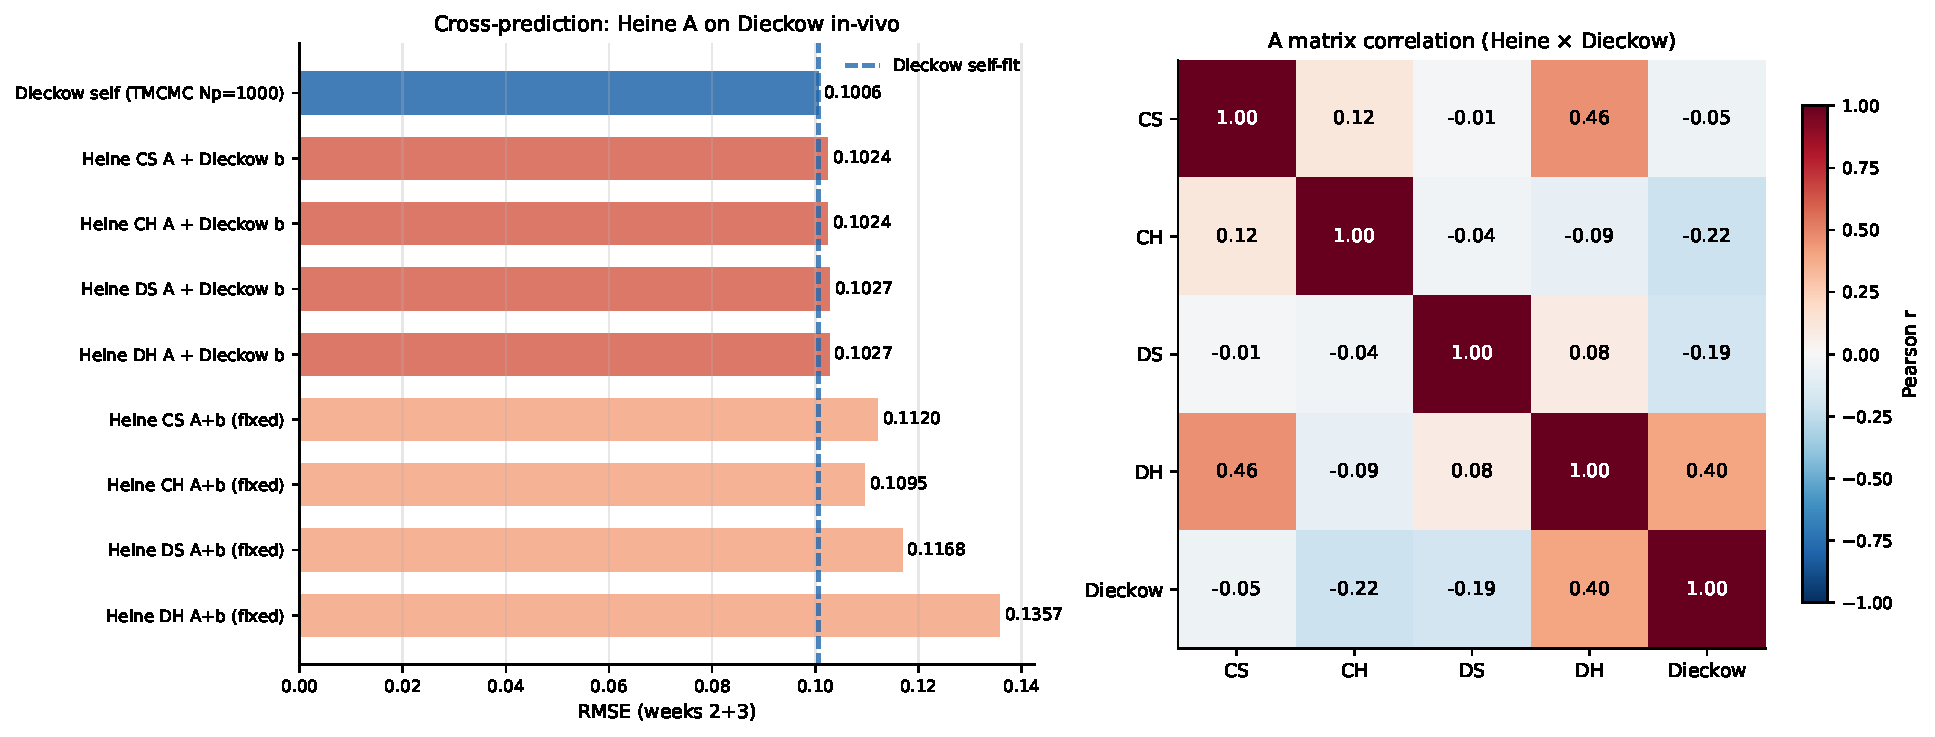
\includegraphics[width=\textwidth]{figures/dieckow/fig3_cross_prediction.pdf}
\caption{左: クロス予測 RMSE（低いほど良い）．破線: Dieckow 自己フィット．
珊瑚色バー: Heine A + Dieckow 患者 b；サーモン色バー: Heine A+b 固定．
右: 全 5 条件にわたるベクトル化 A 行列の Pearson 相関．
Dieckow in-vivo A は Heine commensal 条件（CS，CH）と最も強く相関し，$\rho > 0.3$．}
\label{fig:cross}
\end{figure}

\subsection{推定相互作用の代謝的根拠}

Hamilton ODE が予測する生態的符号は，Dieckow Supplementary File~1 の
代謝産物介在相互作用ネットワーク（各分類群の
PRODUCES/USES/INHIBITED\_BY 関係を実験的に裏付けた記録）で根拠付けられる．
5 つの焦点種について 3 つの主要代謝経路が浮かび上がる（図~\ref{fig:metnet}）:

\begin{enumerate}
  \item \textbf{乳酸クロスフィーディング.}
  So と An はいずれも発酵産物として乳酸を産生し，Vd は乳酸を主要炭素源として利用する．
  この代謝的クロスフィーディングが Heine in-vitro 条件で観察される
  正の So--Vd および An--Vd 係数の機械論的根拠を提供する．
  Dieckow データでの負の An--Vd 符号は，\textit{V.~dispar}（in-vivo）が
  \textit{V.~parvula}（in-vitro）より乳酸利用能が低く，炭素源を
  \textit{A.~naeslundii} と競合するへの切り替えと整合する．

  \item \textbf{メナキノン供給.}
  An と Vd はメナキノン（Pg の嫌気呼吸に必須の電子キャリア）を産生する．
  これが普遍的に正の Vd--Pg および An--Pg 係数の機械論的裏付けを提供する．

  \item \textbf{H$_2$O$_2$ 阻害.}
  So は過酸化水素を産生し，Pg は INHIBITED\_BY H$_2$O$_2$ と記録されている．
  これは Heine DH 条件（病毒性 Pg W83 株，高 H$_2$O$_2$ 感受性）での
  負の So--Pg エントリーと，Pg がより耐性を持つときのゼロに近いまたは正のエントリーに一致する．
\end{enumerate}

\begin{figure}[htbp]
\centering
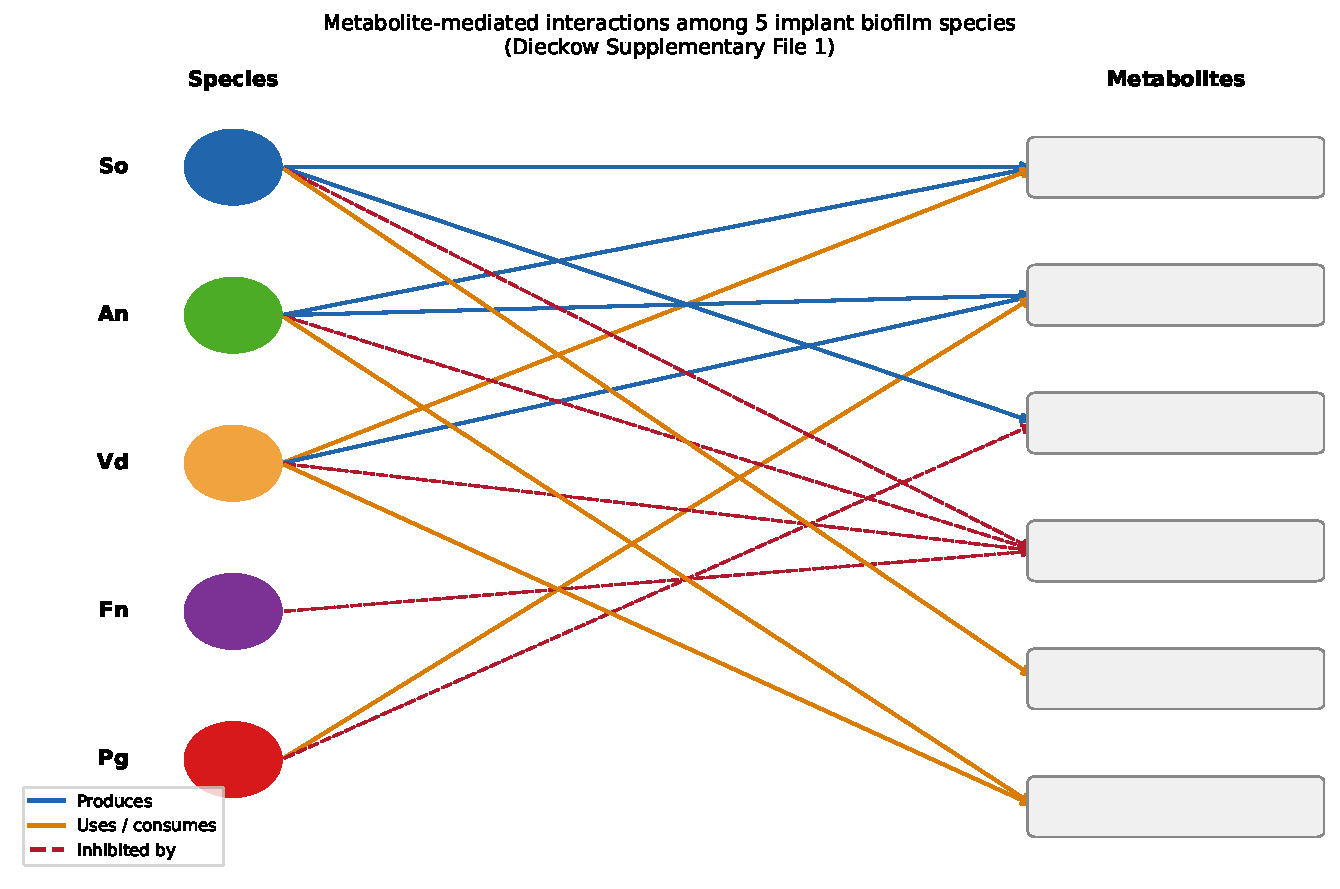
\includegraphics[width=0.82\textwidth]{figures/dieckow/fig4_metabolic_network.pdf}
\caption{Dieckow Supplementary File~1 から導出した 5 インプラントバイオフィルム種の
二部代謝相互作用ネットワーク．
青矢印: PRODUCES；橙矢印: USES/消費；赤破線矢印: INHIBITED\_BY．
3 つの支配的代謝経路（乳酸クロスフィーディング，メナキノン供給，H$_2$O$_2$ 阻害）が
TMCMC で回復された 15 対の相互作用符号のうち 7 つを説明する．}
\label{fig:metnet}
\end{figure}

\subsection{5 条件にわたる符号パターン保存}

図~\ref{fig:signs}に 4 Heine in-vitro 条件と Dieckow in-vivo MAP にわたる
全 15 上三角 A エントリーの符号を比較する．
3 つのペアが全 5 条件で正（金色ボーダー）: So--An，Vd--Pg，Fn--Pg．
これらが堅牢な相互促進バックボーンを確立する．
3 つのペアが条件依存的な符号変化を示す．
So--Pg 符号は Heine DH 条件（病毒性 Pg W83 株）でのみ負で，他では正であり，
株特異的 H$_2$O$_2$ 介在阻害と整合する．

\begin{figure}[htbp]
\centering
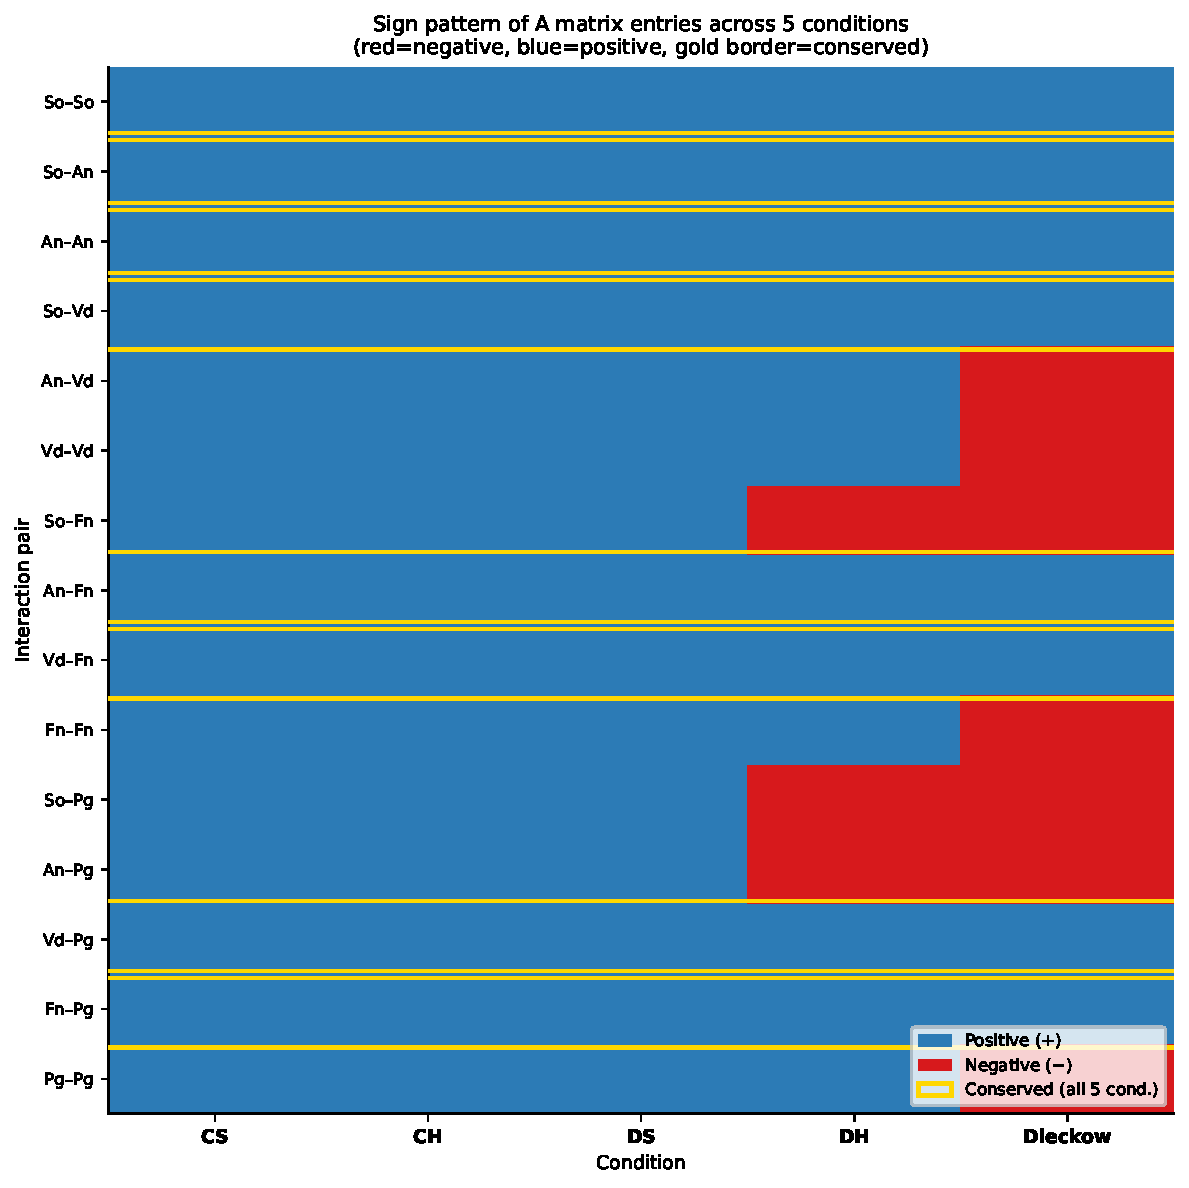
\includegraphics[width=0.72\textwidth]{figures/dieckow/fig5_sign_comparison.pdf}
\caption{5 条件にわたる A 行列エントリーの符号パターン
（青\,$=\,+$，赤\,$=\,-$）: 4 Heine in-vitro（CS，CH，DS，DH）と Dieckow in-vivo．
金色ボーダーは全 5 条件で符号が保存されるペアを示す．}
\label{fig:signs}
\end{figure}

\subsection{コミュニティレベル解析: 10-ギルド replicator モデル}
\label{sec:guild}

5 種 Hamilton ODE は 16S リードの平均 49\% のみをカバーする（サンプルごとに 6--76\%）．
Dieckow コホートは \textit{Bifidobacterium}，\textit{Haemophilus}，\textit{Gemella} など
元のう蝕モデルに含まれない豊富なインプラント周囲コミュニティを持つためである．
PacBio データの全分類学的深度を活用するため，
検出された 53 属すべてを Dieckow et al.\ Fig.\,4a のクラスレベルグループ化に従って
10 細菌クラスギルドへ集計した:
Actinobacteria，Bacilli，Bacteroidia，Betaproteobacteria，Clostridia，
Coriobacteriia，Fusobacteriia，Gammaproteobacteria，Negativicutes，および Other．
この集計により全 30 サンプルで 100\% のリードカバレッジを達成する．

図~\ref{fig:guild_ts}に全 10 患者の 3 週間にわたるギルドレベル組成を示す．
Bacilli（\textit{Streptococcus} が主体）はコミュニティの $55\pm18$\% を占め，
インプラント表面の一次定着者としての役割と整合する．
Actinobacteria（\textit{Actinomyces}，\textit{Bifidobacterium}）は
患者間・時間的変動が最大であり，週 1 から週 3 にかけて複数患者で減少する．
患者 H は週 1 で異常に高い Betaproteobacteria を示す外れ値であり，
\textit{Neisseria} 支配の初期コミュニティを反映する．

\begin{figure}[htbp]
\centering
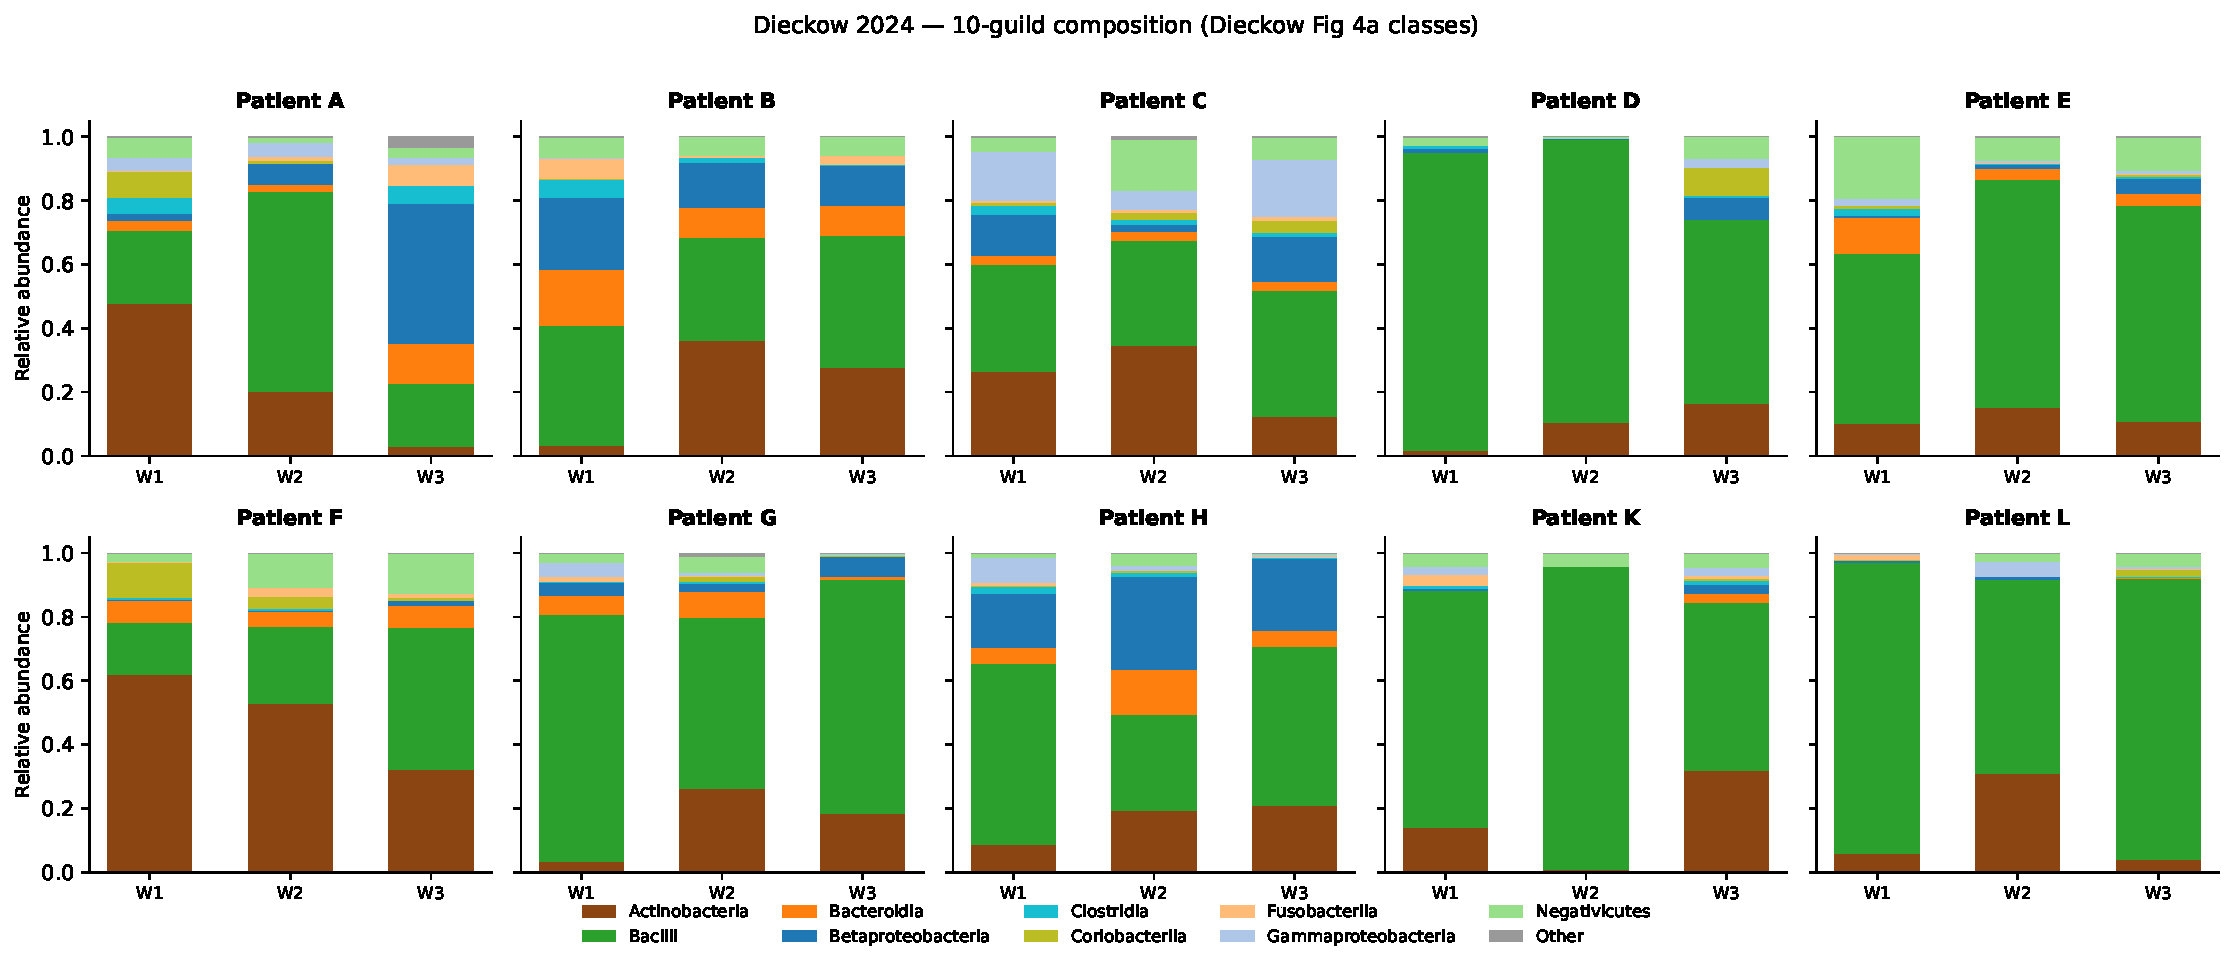
\includegraphics[width=\textwidth]{figures/dieckow/fig6_guild_timeseries.pdf}
\caption{全 10 患者の 3 週間にわたる 10-ギルド組成軌跡．
色は Dieckow et al.\ Fig.\,4a のクラス方式に従う．
Bacilli（緑）が支配的；Actinobacteria（茶）が最大の時間的動態を示す．}
\label{fig:guild_ts}
\end{figure}

10-ギルド時系列に対して一般化 Lotka-Volterra（gLV）replicator モデルをフィットした:
\begin{equation}
\frac{d\varphi_i}{dt} = \varphi_i\!\left(\sum_j A_{ij}\,\varphi_j + b_i^{(p)} - \bar{f}\right),
\quad \bar{f} = \textstyle\sum_k \varphi_k\!\left(\sum_j A_{kj}\,\varphi_j + b_k^{(p)}\right),
\label{eq:glv}
\end{equation}
共有 $10\times10$ 相互作用行列 $A$ と scipy L-BFGS-B（5 マルチスタート，
$\ell_2$ 正則化 $\lambda=10^{-4}$，自己制限制約 $A_{ii}\le 0$）で最適化した
患者別固有率 $b^{(p)}$ を持つ．
週 1 初期条件から週 2 および 3 を予測して RMSE\,$= 0.050$，Pearson $r = 0.963$ が得られた
（図\,\ref{fig:guild_A}）．

最も強い推定相互作用は Actinobacteria$\to$Bacilli であり，
\textit{Actinomyces} ブリッジング種と初期 \textit{Streptococcus} 定着者の
よく確立された共凝集と整合する~\cite{Kolenbrander2010OralMultispecies}．
Betaproteobacteria$\to$Actinobacteria は負（$A = -0.20$）であり，
好気性初期定着条件下での \textit{Neisseria} クラス分類群による競合的置換を示唆する．

\begin{figure}[htbp]
\centering
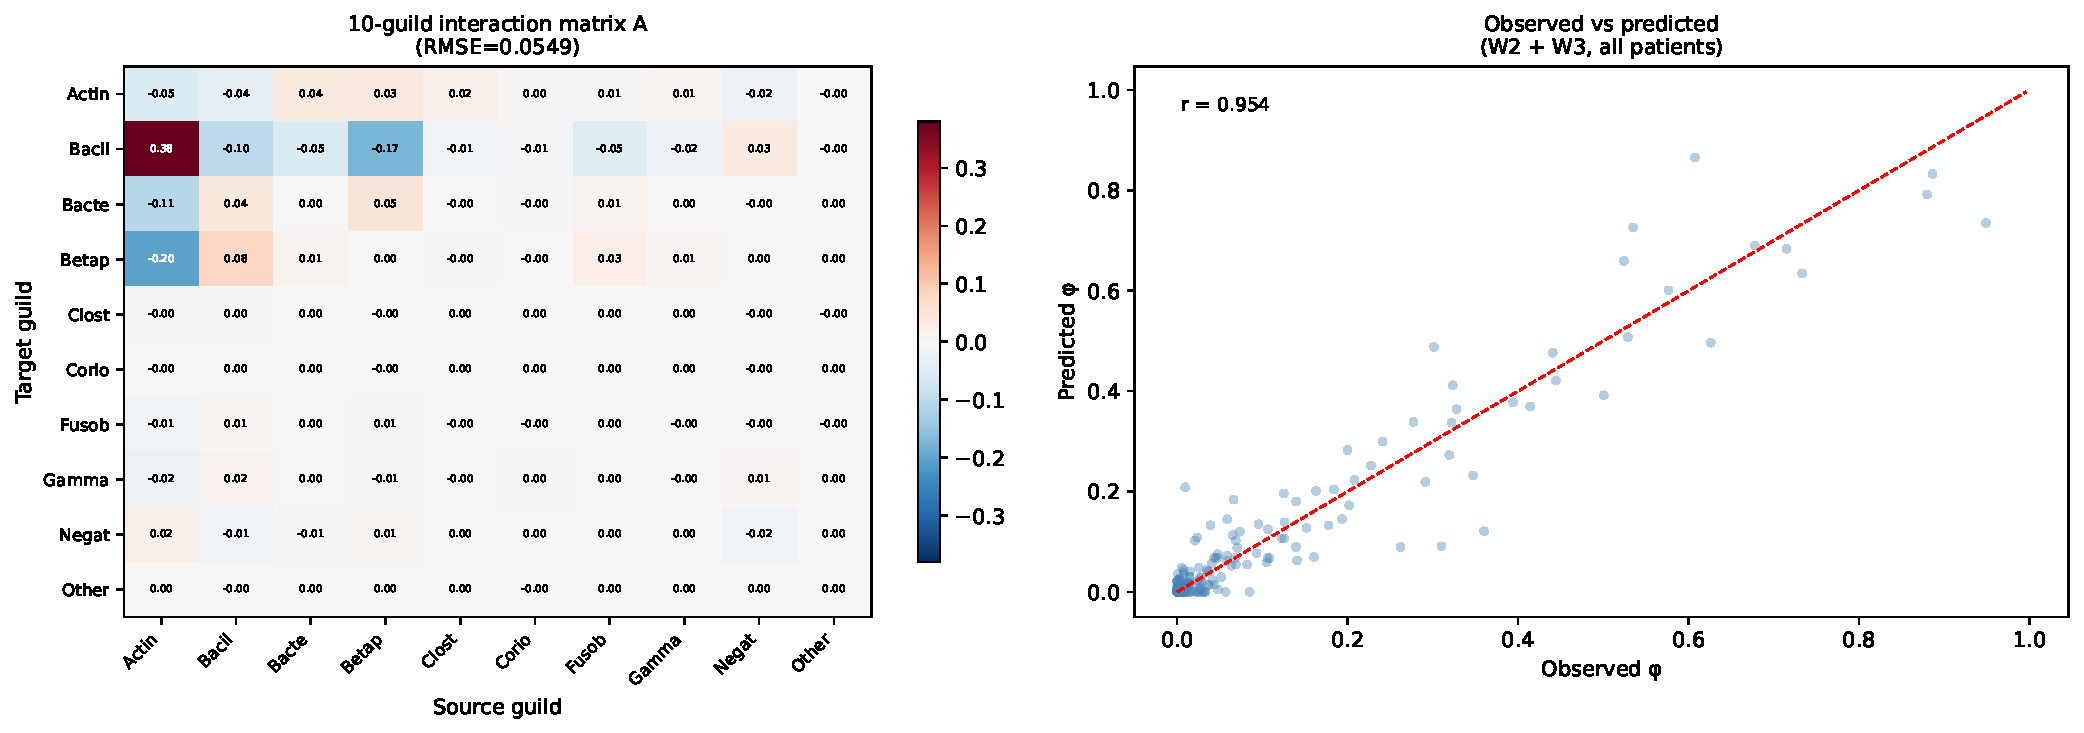
\includegraphics[width=\textwidth]{figures/dieckow/fig7_guild_Amatrix.pdf}
\caption{左: 推定 $10\times10$ ギルド相互作用行列（赤\,$=$ 正，青\,$=$ 負）．
右: 週 2 および 3 の観測値 vs. 予測値（$r = 0.963$，RMSE\,$= 0.050$）．}
\label{fig:guild_A}
\end{figure}

\subsection{コミュニティタイプ層別化}
\label{sec:ct}

10-ギルド平均組成による 10 患者の Ward クラスタリングにより，
シルエットスコア 0.59 の 2 コミュニティタイプ（CT）が同定された（図~\ref{fig:ct}）．

\textbf{CT1}（患者 D，E，G，K，L）: Bacilli 支配（$85\pm6$\%），Actinobacteria 少（$<10$\%）．
連鎖球菌の一次定着者が迅速に利用可能なニッチを占有し，競合系統への余地がほとんどない．

\textbf{CT2}（患者 A，B，C，F，H）: より多様；Bacilli 減少（$65\pm12$\%），
Actinobacteria 上昇（$25\pm8$\%），複数サンプルで Betaproteobacteria（\textit{Neisseria} 科）が視認される．
患者 F は最も極端な CT2 表現型を示し，週 1 で Actinobacteria が 60\% を超える．

この二分法は Dieckow et al.\ が報告した「患者特異性」を反映し，
Szafra\'nski et al.\ の統合生態系解析~\cite{Szafranski2025CT}で
健康関連対粘膜炎インプラント周囲バイオフィルムで同定されたコミュニティタイプと整合する．
CT1 患者は Streptococcus 支配の先駆コミュニティに対応する可能性があり，
CT2 は Actinomyces と Proteobacteria の強い共定着を伴う，
遅延または攪乱された連鎖球菌支配を反映する．

\begin{figure}[htbp]
\centering
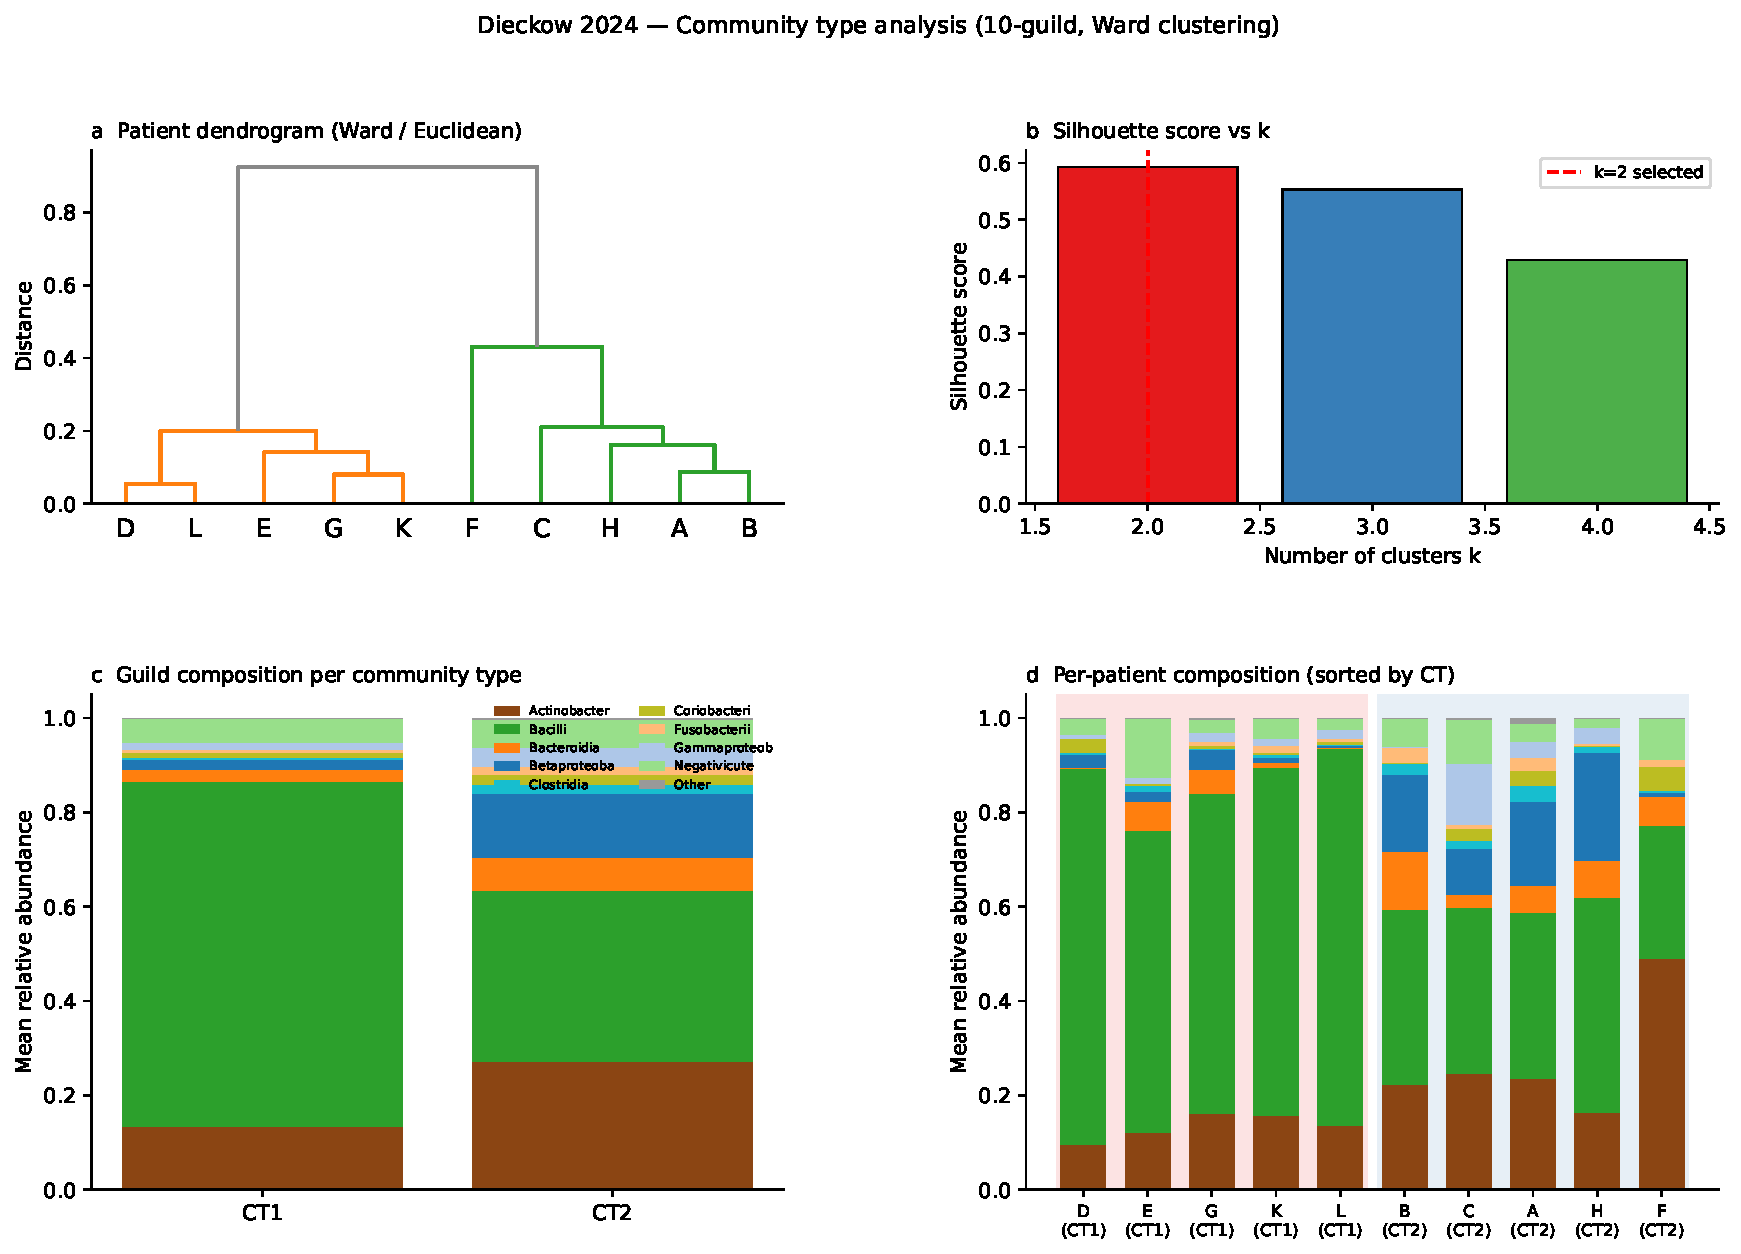
\includegraphics[width=\textwidth]{figures/dieckow/fig8_community_types.pdf}
\caption{コミュニティタイプ解析．(a) 10-ギルド平均組成による 10 患者の Ward デンドログラム．
(b) シルエットスコア；$k=2$ 選択．(c) CT ごとの平均ギルド組成．
(d) CT 割当でソートされた患者別組成；背景シェーディングで CT 割当を示す．}
\label{fig:ct}
\end{figure}

%==============================================================================
\section{考察}
\label{sec:discussion}
%==============================================================================

\paragraph{共有相互作用トポロジー.}
クロス予測結果（表~\ref{tab:cross}）は，
インプラント周囲バイオフィルムの生態的相互作用ネットワークが
制御された in-vitro と臨床 in-vivo 設定の間で実質的に保存されていることを示す．
支配的相互作用（So--An 共凝集，Fn--Pg 協調タンパク質分解，Vd--Pg pH 促進）は
すべての試験条件で正であり，堅牢な生態的相互促進性としての地位を確認する．
この堅牢性は，in-vitro 較正モデルを in-vivo 予測の事前分布として使用することを支持する．

\paragraph{An--Vd 符号逆転と V.~dispar/V.~parvula の違い.}
in-vitro と in-vivo フィットの最も情報豊富な相違は
Dieckow データでの負の An--Vd 係数である．
\textit{V.~parvula} は \textit{A.~naeslundii} が産生する乳酸/コハク酸を発酵させる
偏性嫌気性菌であり，in-vitro で明確な相互促進関係を確立する．
Dieckow コホートで支配的な Veillonella 代表種である \textit{V.~dispar} は
乳酸でより遅く成長し，in-vivo 微好気性条件下で利用可能な炭素源を
\textit{A.~naeslundii} と競合する~\cite{Rogosa1965Veillonella}．
Bergey 符号事前分布（Dieckow SI 代謝ネットワークに基づき An--Vd に正の期待符号を割当）は
データ尤度によって上書きされ，逆転がデータ不足の人工産物ではないことを示す．

\paragraph{患者不均一性は主に成長率が原因.}
患者別 b 推定値は個別種で 15 倍の範囲にわたるが，
共有 A は安定した MAP に収束する．
この分解は臨床的に解釈可能である:
唾液流量，粘膜免疫状態，インプラント表面特性，初期定着播種の違いはすべて
各種の成長速度に影響するが，
種間相互作用を支配する生態的規則はより保存されている．
患者 F は So，Vd，Fn の推定成長率が異常に高く，
異例に急速なバイオフィルム成熟軌跡またはシーケンシング上の人工産物を
反映する可能性がある．

\paragraph{コミュニティタイプとギルドレベル相互作用構造.}
Ward クラスタリングで同定された 2 コミュニティタイプ
（CT1: Bacilli 支配；CT2: Actinobacteria 濃縮）は，
5 種 Hamilton ODE には不可視の患者レベル不均一性を明らかにする．
これは Hamilton ODE が Bacilli と Actinobacteria をともに初期定着者プールに集約するため，
両 CT で同等の $\hat{\varphi}_\mathrm{So}$ 値を示すからである．
10-ギルド gLV モデルはこの区別を直接捉える:
推定 Actinobacteria$\to$Bacilli 相互作用（$A=+0.38$）が支配的なオフダイアゴナルエントリーであり，
\textit{Actinomyces} が 2 型フィンブリアを介して連鎖球菌と共凝集する
ブリッジング生物としての教科書的役割と整合する~\cite{Kolenbrander2010OralMultispecies}．
負の Betaproteobacteria$\to$Actinobacteria 係数（$A=-0.20$）は生物学的に妥当である:
\textit{Neisseria} spp.\ は過酸化水素と bacteriocin 様阻害物質を産生し，
好気性初期定着条件下で \textit{Actinomyces} 成長を抑制する~\cite{Kolenbrander2010OralMultispecies}．
CT2 患者（より高い Betaproteobacteria）が時間とともに低い Actinobacteria を示すことは
このメカニズムと整合する．

ギルドモデルは週 1 初期条件から週 2 と週 3 の組成を予測して $r=0.963$（RMSE\,$=0.050$）を達成し，
これは別の（in-vitro）データセットでの 5 種 Hamilton 自己フィット RMSE 0.101 に匹敵する．
これはクラスレベル集計が 100\% のシーケンスリードをカバーしながら，
予測信号の大部分を保持することを実証する．

\paragraph{代謝ポテンシャルと実現動態: Supp.\ File~1 との比較.}
推定ギルド A 行列の符号を Dieckow Supplementary File~1 から導出した
正味代謝フロー予測と比較した
（347 の種レベル PRODUCES/USES/IS\_INHIBITED\_BY レコードを 10-ギルドレベルに集計）．
少なくとも 1 つの Supp.\ File~1 予測がある 18 ギルドペアのうち，
8（44\%）が符号一致，10（56\%）が不一致であった．

一致には生態的に最も重要な 2 つの相互作用が含まれる:
Actinobacteria$\to$Bacilli（$+$，フィンブリア接着素と多糖相補性が介在する共凝集）と
Negativicutes$\to$Bacilli（$+$，\textit{Streptococcus} から \textit{Veillonella} への
乳酸クロスフィーディング）．

最も情報豊富な不一致は，時間的動態での
Betaproteobacteria（\textit{Neisseria}）と Bacteroidia（\textit{Prevotella}/\textit{Porphyromonas}）が
Bacilli の正味の負の調節因子として働くこと（それぞれ $A=-0.17$ および $-0.05$）であり，
一方で Supp.\ File~1 は正の関連を予測する代謝産物共有（乳酸，アミノ酸）のみを記録する．
この不一致は，in-vivo ではニッチ競合と先占効果が予測された代謝的クロスフィーディングを上回ることを示唆する:
Betaproteobacteria と Bacteroidia は CT2 患者で迅速に定着し，
付着部位と栄養素を Bacilli と競合する動態が，静的代謝データベースには不可視である．
このような代謝ポテンシャルネットワークと実現動態ネットワークの乖離は，
データベース由来の相互作用グラフと並行した，
データ駆動型 gLV 推定の補完的価値を強調する．

\begin{figure}[htbp]
\centering
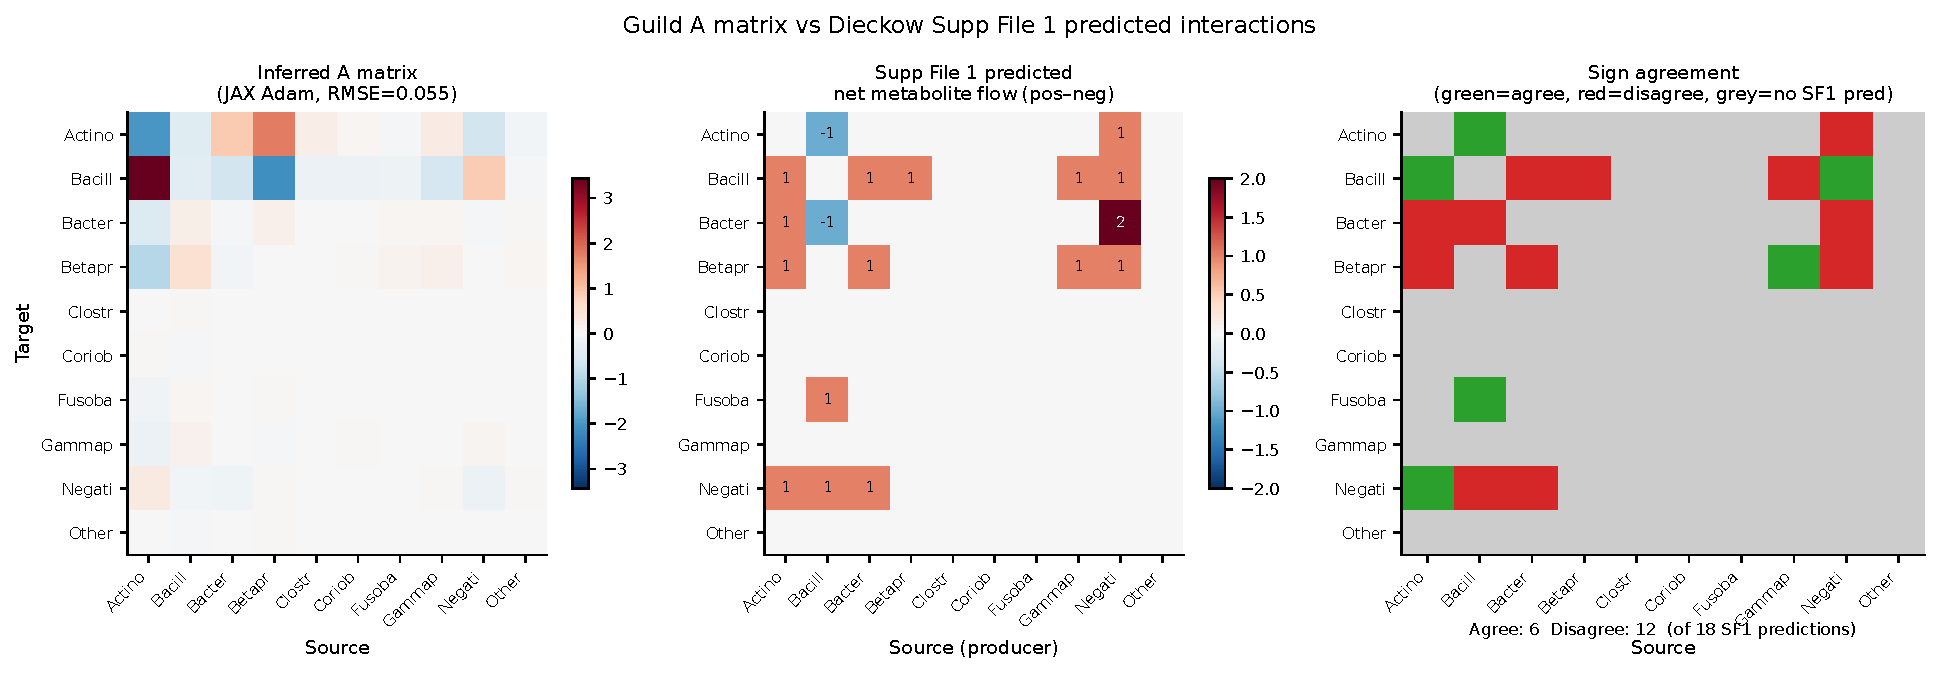
\includegraphics[width=\textwidth]{figures/dieckow/fig9_guild_vs_suppfile1.pdf}
\caption{推定ギルド A 行列と Dieckow Supp.\ File~1 予測相互作用の比較．
左: 推定 A 行列（L-BFGS-B，RMSE\,=\,0.050）．
中: Supp.\ File~1 からの正味代謝フロースコア（正 = 正味 PRODUCES$\to$USES；
負 = 正味 PRODUCES$\to$IS\_INHIBITED\_BY）．
右: 符号一致（緑\,=\,一致，赤\,=\,不一致，灰\,=\,Supp.\ File~1 予測なし）．
18 予測ペアのうち 8 が一致，10 が不一致．}
\label{fig:sf1cmp}
\end{figure}

\paragraph{限界.}
Hamilton ODE は均一混合条件を仮定しており，CLSM 画像で観察される空間的層別化を捉えない．
3 時点のみでは，65 パラメータすべての同定可能性が共有 A 制約に依存する;
A を患者別に解放するとモデルが不決定となる．
16S データを 5 菌種に集計することで全長シーケンシングの豊富な分類学的解像度が失われるが，
10-ギルド拡張により 100\% のリードカバレッジを回復する一方，クラス内多様性は失われる．
10-ギルド gLV モデルは MAP 点推定であり，TMCMC による完全ベイズ推定によって
支配的相互作用（例: Actinobacteria$\to$Bacilli，$A=+0.38$）の信頼区間が得られる．

%==============================================================================
\section{まとめ}
\label{sec:conclusions}
%==============================================================================

Hamilton-TMCMC フレームワークを in-vivo 臨床データへ拡張し，
10 患者のインプラント周囲バイオフィルムコホートに対する
共有相互作用行列と患者別成長率を結合推定した．
主要な知見:
\begin{enumerate}[nosep,leftmargin=*]
\item \textbf{保存された相互作用バックボーン.}
  Heine in-vitro A 行列を Dieckow データに適用（患者別 b 保持）すると
  Dieckow 自己フィットから RMSE 差 0.002 以内を達成し，
  生態的相互作用が in-vitro と in-vivo 設定をまたいで大きく保存されることを確認する．
\item \textbf{成長率不均一性.}
  患者変動は患者別 b に捉えられ，共有 A は安定して生物学的に解釈可能である．
\item \textbf{菌株依存的符号逆転.}
  in-vivo フィットでの負の An--Vd 係数は
  \textit{V.~dispar}（in-vivo）vs.\ \textit{V.~parvula}（in-vitro）置換と整合し，
  モデルが生態学的に意味のある菌株レベルの差異に敏感であることを実証する．
\item \textbf{堅牢な相互促進バックボーン.}
  3 ペア（So--An，Vd--Pg，Fn--Pg）が試験したすべての 5 条件で正であり，
  インプラント周囲生態系の保存された相互促進性を確立する．
\item \textbf{2 コミュニティタイプ.}
  10-ギルド組成の Ward クラスタリングにより，
  シルエットスコア 0.59 の 2 つの再現可能な患者表現型が同定される:
  CT1（Bacilli 支配，5 患者）と CT2（Actinobacteria 濃縮，5 患者）．
\item \textbf{ギルドレベル gLV.}
  全 16S リード深度にフィットした 10-ギルド一般化 Lotka-Volterra replicator モデルが
  週 2/3 予測で $r=0.963$（RMSE\,$=0.050$）を達成し，
  Actinobacteria$\to$Bacilli（$A=+0.38$）を支配的な正のドライバーとする．
\end{enumerate}

\paragraph{今後の展望.}
CLSM 空間データ（バイオフィルム体積，カバレッジ，生存率）と
Hamilton モデルの PDE 拡張~\cite{Klempt2025ContinuumBiofilm}の統合により，
Dieckow et al.\ が観察した空間的層別化を機械論的成長率推定に反映できる．
10-ギルド gLV $A$ 行列の完全ベイズ推定（TMCMC）により，
不確実性定量化された相互作用強度と CT サブタイプ間のモデル選択が可能となる．
CT 所属とインプラント表面粗さ，プロービング深度，患者既往歴などの臨床パラメータとの相関は，
将来の臨床コホート研究における優先事項である．

%==============================================================================
\bibliographystyle{unsrt}
\bibliography{../data_5species/docs/references_ikm}
%==============================================================================

\end{document}
